%\section{Sở GD Lạng Sơn --Lần 1 NH: 2025--2026}
\vspace{-0.5cm}
\Opensolutionfile{ans}[ans/ans-26-2-LangSon-SoGD-L1]
\caulc

\begin{ex}%[1D2H2-4]%Câu 1
	Cho cấp số cộng $(u_n)$ có $u_1=1$, $u_2=4$. Số hạng thứ tư là
	\choice
	{$u_4=9$}
	{$u_4=12$}
	{$u_4=13$}
	{\True $u_4=10$}
	\loigiai{
		Công sai của cấp số cộng là $d=u_2-u_1=4-1=3$.\\
		Số hạng thứ tư là $u_4=u_1+3d=1+3\cdot 3=10$.
	}
\end{ex}

\begin{ex}%[2H2N2-1]%Câu 2
	Trong không gian, cho hình hộp $ABCD.EFGH$. Mệnh đề nào sau đây đúng?
	\choice
	{\True $\overrightarrow{AB}+\overrightarrow{AD}+\overrightarrow{AE}=\overrightarrow{AG}$}
{$\overrightarrow{DA}+\overrightarrow{DC}+\overrightarrow{DE}=\overrightarrow{DF}$}
{$\overrightarrow{BA}+\overrightarrow{BC}+\overrightarrow{BE}=\overrightarrow{BH}$}
{$\overrightarrow{EA}+\overrightarrow{EF}+\overrightarrow{EB}=\overrightarrow{EC}$}
	\loigiai{
		Theo quy tắc hình hộp ta có $\overrightarrow{AB}+\overrightarrow{AD}+\overrightarrow{AE}=\overrightarrow{AG}$.
	}
\end{ex}

\begin{ex}%[1D5V2-3]%Câu 3
	Một học sinh tiến thành thống kê nhiệt độ trung bình tại nơi mình sống trong vòng $40$ ngày và thu được bảng số liệu sau:
	\begin{center}
\begin{tabular}{|c|c|c|c|c|}
\hline 
Nhiệt độ ($^\circ C$) & $[19;22)$ & $[22;25)$ & $[25;28)$ & $[28;31)$ \\ 
\hline 
Số ngày & $7$ & $15$ & $12$ & $6$ \\ 
\hline 
\end{tabular} 
\end{center}

	Tứ phân vị thứ nhất của bảng số liệu trên bằng
	\choice
	{$23{,}5$}
	{$27$}
	{$26{,}5$}
	{\True $22{,}6$}
	\loigiai{
		Cỡ mẫu là $N=40$. Tứ phân vị thứ nhất $Q_1$ là giá trị thuộc nhóm đầu tiên có tần số tích lũy lớn hơn hoặc bằng $\dfrac{40}{4}=10$.\\
		Vì nhóm $[22;25)$ có tần số tích lũy $7+15=22 \geq 10$ nên $Q_1\in[22;25)$.\\
		Vậy $Q_1 = 22 + \dfrac{10-7}{15}\cdot 3 = 22 + \dfrac{3}{15}\cdot 3 = 22 + 0{,}6 = 22{,}6$.
	}
\end{ex}

\begin{ex}%[1D1H5-3]%Câu 4
	Nghiệm của phương trình $\cos 2x=1$ là
	\choice
	{\True $x=k\pi, k\in\mathbb{Z}$}
	{$x=\pi+k2\pi, k\in\mathbb{Z}$}
	{$x=\dfrac{\pi}{2}+k\pi, k\in\mathbb{Z}$}
	{$x=\pi+k\pi, k\in\mathbb{Z}$}
	\loigiai{
		$\cos 2x=1 \Leftrightarrow 2x=k2\pi \Leftrightarrow x=k\pi, k\in\mathbb{Z}$.
	}
\end{ex}

\begin{ex}%[1D6H2-3]%Câu 5
	Với $a$ là số thực dương tùy ý, $\log_3(9a)$ bằng
	\choice
	{$3+a$}
	{\True $2+\log_3 a$}
	{$3+\log_3 a$}
	{$2\log_3 a$}
	\loigiai{
		$\log_3(9a) = \log_3 9 + \log_3 a = 2 + \log_3 a$.
	}
\end{ex}

\begin{ex}%[2D1N1-2]%Câu 6
	Cho hàm số $y=f(x)$ có đồ thị như bên dưới. 
	 \begin{center}
	 \begin{tikzpicture}[scale=1,font=\footnotesize, line cap=round,line join=round,>=stealth]
\draw[->, thick] (-3.0,0) -- (3.4,0) node[above] {$x$};
\draw[->, thick] (0,-4.8) -- (0,4.8) node[left] {$y$};
\draw[thick] (-3.,-3.0) -- (3.2,3.2);
\draw[thick, smooth, domain=0.22:3.1, samples=300]
  plot (\x, {\x + 1/\x});
\draw[thick, smooth, domain=-3.0:-0.22, samples=300]
  plot (\x, {\x + 1/\x});
\draw[dashed, thick] (0,2) -- (1,2);
\draw[dashed, thick] (1,0) -- (1,2);
\draw[dashed, thick] (-1,0) -- (-1,-2);
\draw[dashed, thick] (-1,-2) -- (0,-2);
\node[above] at (-1,0) {$-1$};
\node[below right] at (0,0) {$O$};
\node[below] at (1,0) {$1$};
\node[below] at (2,0) {$2$};
\node[left]  at (0,2) {$2$};
\node[right] at (0,-2) {$-2$};
\end{tikzpicture}
	 	\end{center}	
	Hàm số đã cho nghịch biến trên khoảng nào trong các khoảng sau đây?
	\choice
	{$(0;2)$}
	{$(-1;1)$}
	{\True $(-1;0)$}
	{$(1;2)$}
	\loigiai{
		Dựa vào đồ thị, trên khoảng $(-1;0)$, đồ thị hàm số đi xuống từ trái sang phải, do đó hàm số nghịch biến trên $(-1;0)$.
	}
\end{ex}

\begin{ex}%[1H4N3-2]%Câu 7
	Cho hình chóp $S.ABC$. Gọi $I, J$ lần lượt là trung điểm của các cạnh $SA, SB$. Khẳng định nào dưới đây đúng?
	\choice
	{$IJ \parallel (SAB)$}
	{$IJ \parallel (SAC)$}
	{\True $IJ \parallel (ABC)$}
	{$IJ \parallel (SBC)$}
	\loigiai{
		Vì $IJ$ là đường trung bình trong tam giác $ABC$ nên $IJ \parallel AB$.\\
		Mà $AB \subset (ABC)$ nên $IJ \parallel (ABC)$.
	}
\end{ex}

\begin{ex}%[2D4N1-3]%Câu 8
	Họ nguyên hàm của hàm số $f(x)=\sin x$ là
	\choice
	{$F(x)=-\tan x+C$}
	{$F(x)=\cos x+C$}
	{\True $F(x)=-\cos x+C$}
	{$F(x)=\tan x+C$}
	\loigiai{
		Ta có $\displaystyle\int \sin x \mathrm{\,d}x = -\cos x + C$.
	}
\end{ex}

\begin{ex}%[2H5N1-2]%Câu 9
	Trong không gian $Oxyz$, cho mặt phẳng $(P)\colon 2x-y+4z-1=0$. Một vectơ pháp tuyến của $(P)$ là
	\choice
	{$\vec{n}_3=(2;1;4)$}
	{$\vec{n}_4=(2;4;-1)$}
	{\True $\vec{n}_1=(-2;1;-4)$}
	{$\vec{n}_2=(2;-1;-1)$}
	\loigiai{
		Mặt phẳng $(P)$ có một vectơ pháp tuyến là $\vec{n}=(2;-1;4)$.\\
		Vectơ $\vec{n}_1=(-2;1;-4) = -\vec{n}$ cũng là một vectơ pháp tuyến.
	}
\end{ex}

\begin{ex}%[1H8N2-2]%Câu 10
	Cho hình chóp $S.ABCD$ có đáy $ABCD$ là hình thoi tâm $O$, $SA=SC, SB=SD$. Trong các khẳng định sau khẳng định nào đúng?
	\choice
	{$SC \perp (ABCD)$}
	{\True $SO \perp (ABCD)$}
	{$SB \perp (ABCD)$}
	{$SA \perp (ABCD)$}
	\loigiai{
		Vì $SA=SC$ nên tam giác $SAC$ cân tại $S$, suy ra $SO \perp AC$ ($O$ là trung điểm $AC$).\\
		Vì $SB=SD$ nên tam giác $SBD$ cân tại $S$, suy ra $SO \perp BD$ ($O$ là trung điểm $BD$).\\
		Do $SO \perp AC$ và $SO \perp BD$ nên $SO \perp (ABCD)$.
	}
\end{ex}

\begin{ex}%[2H2N2-3]%Câu 11
	Trong không gian $Oxyz$, cho các vectơ $\vec{u}=(1;-2;2)$ và $\vec{v}=(1;3;-5)$. Tọa độ của vectơ $\vec{w}=\vec{u}-\vec{v}$ là
	\choice
	{$(2;1;-3)$}
	{$(0;1;-3)$}
	{\True $(0;-5;7)$}
	{$(0;5;-7)$}
	\loigiai{
		$\vec{w} = (1-1; -2-3; 2-(-5)) = (0;-5;7)$.
	}
\end{ex}

\begin{ex}%[2D4N2-1]%Câu 12
	Cho hàm số $f(x)$ liên tục trên $\mathbb{R}$, thỏa mãn $\displaystyle\int\limits_0^4 f(x)\mathrm{\,d}x=-3$ và $\displaystyle\int\limits_4^3 f(x)\mathrm{\,d}x=2$. Khi đó, $\displaystyle\int\limits_0^3 f(x)\mathrm{\,d}x$ bằng 
	\choice
	{$-5$}
	{\True $-1$}
	{$1$}
	{$5$}
	\loigiai{
	Vì $\displaystyle\int\limits_4^3 f(x)\mathrm{\,d}x=2$ nên $\displaystyle\int\limits_3^4 f(x)\mathrm{\,d}x=-2$ .\\		
		Ta có $\displaystyle\int\limits_0^4 f(x)\mathrm{\,d}x = \displaystyle\int\limits_0^3 f(x)\mathrm{\,d}x+\displaystyle\int\limits_3^4 f(x)\mathrm{\,d}x$.\\
		Suy ra $\displaystyle\int\limits_0^3 f(x)\mathrm{\,d}x=\displaystyle\int\limits_0^4 f(x)\mathrm{\,d}x-\displaystyle\int\limits_3^4 f(x)\mathrm{\,d}x=-3-(-2)=-1$. 
	}
\end{ex}
\Closesolutionfile{ans}

\cauds
\Opensolutionfile{ans}[ans/ans-26-2-LangSon-SoGD-L1-DS]
\begin{ex}%[2D4V2-6]%Câu 1
	Giả sử rằng khi được $t$ năm tuổi, một máy công nghiệp $A$ tạo ra doanh thu với tốc độ $R^{\prime}(t)=588-3t^2$ (triệu đồng/năm), thời điểm $t=0$ tính từ lúc máy $A$ bắt đầu hoạt động. Biết rằng chi phí biên cho vận hành và bảo trì là $C^{\prime}(t)=48+12t^2$ (triệu đồng/năm), ở đây $C(t)$ là chi phí vận hành và bảo trì máy $A$ khi nó được $t$ năm tuổi. Khi đó:
	\choiceTF
	{\True Doanh thu sau 10 năm của máy $A$ là $\displaystyle\int\limits_0^{10}(588-3t^2)\mathrm{\,d}t$ (triệu đồng)}
	{\True Tổng chi phí vận hành và bảo trì của máy $A$ trong 6 năm là $1\,152$ (triệu đồng)}
	{\True Tuổi thọ hữu ích của một máy là số năm $T$ trước khi lợi nhuận (bằng doanh thu trừ chi phí) mà nó tạo ra bắt đầu giảm. Tuổi thọ hữu ích của máy $A$ này là $8$ năm}
	{Lợi nhuận do máy $A$ tạo ra trong suốt thời gian tuổi thọ hữu ích của nó là $2\,180$ (triệu đồng)}
	\loigiai{
		\begin{itemchoice}
			\itemch \textbf{Đúng.} Doanh thu sau $T$ năm là $\displaystyle\int\limits_0^T R'(t) \mathrm{\,d}t$. Với $T=10$, ta có $\displaystyle\int\limits_0^{10}(588-3t^2)\mathrm{\,d}t$.
			\itemch \textbf{Đúng.} Tổng chi phí trong $6$ năm là $\displaystyle\int\limits_0^6 \left(48+12t^2\right) \mathrm{\,d}t= 1\,152$.
			\itemch \textbf{Sai.} Lợi nhuận do máy $A$ tạo ra là $L(t)=R(t)-C(t)$. Ta có $$L^\prime (t)=R^\prime (t)-C^\prime(t)=588-3t^2 - 48-12t^2=540-15t^2.$$
Ta có $L^\prime(t)=0\Leftrightarrow 540-15t^2\Leftrightarrow t=6$ hoặc $t=-6$. Vì $L^\prime(t)\leq 0$ với mọi $t\in[6;+\infty)$ tuổi thọ hữu ích là $6$ năm.
			\itemch \textbf{Sai.} Lợi nhuận trong $6$ năm là $\displaystyle\int\limits_0^6 \left(R^\prime (t)-C^\prime(t)\right) \mathrm{\,d}t = \displaystyle\int\limits_0^6 (540-15t^2) \mathrm{\,d}t = 2\,160$.
		\end{itemchoice}
	}
\end{ex}

\begin{ex}%[0D0C2-8]%Câu 2
	Có tám bạn học sinh ngồi quanh một cái bàn tròn, mỗi bạn cầm một đồng xu (các đồng xu đều cân đối, đồng chất). Tất cả tám bạn cùng tung đồng xu của mình, bạn nào gieo được mặt ngửa sẽ đứng lên. Khi đó:
	\choiceTF
	{\True Số phần tử của không gian mẫu khi tám bạn cùng tung đồng xu bằng $256$}
	{\True Số kết quả của phép thử sao cho có đúng một bạn đứng lên là $8$}
	{Số kết quả của phép thử sao cho có đúng hai bạn đứng lên, và hai bạn đó không đứng cạnh nhau là $8$}
	{Xác suất có ít nhất hai bạn ngồi liền kề nhau phải đứng lên là $\dfrac{105}{128}$}
	\loigiai{
		\begin{itemchoice}
			\itemch \textbf{Đúng.} Mỗi bạn khi tung đồng xu có thể xảy ra $2$ kết quả sấp hoặc ngửa. Do đó $8$ bạn gieo đồng xu thì có $2^8 = 256$ kết quả.
			\itemch \textbf{Đúng.} Chọn $1$ trong $8$ bạn đứng lên có $\mathrm{C}_8^1 = 8$ cách.
			\itemch \textbf{Sai.} Giả sử có một bạn đứng lên. Khi đó có 5 cách chọn bạn thứ hai không đứng cạnh bạn đang đứng. Suy ra có $8\cdot 5=40$ kết quả mà có đúng hai bạn đứng lên, và hai bạn đó không đứng cạnh nhau. Khi đếm như trên, mỗi hai bạn đứng cạnh nhau được đếm hai lần. Vậy có $20$ kết quả thỏa mãn.
			\itemch \textbf{Sai.} \textbf{Trường hợp 1.} Không có bạn nào đứng lên. Có $1$ cách chọn.\\
			\textbf{Trường hợp $2$.} Có đúng $1$ bạn đứng lên. Có $8$ cách chọn.\\
			\textbf{Trường hợp $3$.} Có đúng $2$ bạn đứng lên và không cạnh nhau. Có $20$ cách chọn (theo ý \textbf{c)}).\\
			\textbf{Trường hợp $4$.} Có đúng $3$ bạn đứng lên, trong đó không có $2$ bạn nào cạnh nhau. Có $\mathrm{C}^3_8$ cách chọn $3$ trong $8$ bạn. Ta đánh số các bạn bởi $1,2,3,\ldots,8$.
			\begin{itemize}
			\item[(1)] Chọn $3$ bạn cạnh nhau. Có $8$ cách chọn, gồm $(1,2,3)$, $(2,3,4),\ldots,(8,1,2)$.
			\item[(2)] Chọn $2$ bạn cạnh nhau và $1$ bạn không cạnh $2$ bạn đã chọn: Có $8$ cách chọn $2$ bạn cạnh nhau (gồm $(1,2), (2,3),\ldots (8,1)$). Cứ mỗi cách chọn $2$ bạn cạnh nhau, có $4$ cách chọn $1$ bạn không cạnh hai bạn đó. Do đó có $8\cdot 4=32$ cách chọn.
			\end{itemize}
			Vậy có $\mathrm{C}^3_8-8-8.4=16$ cách chọn cho trường hợp $4$.\\
			\textbf{Trường hợp $5$.} Có đúng $4$ bạn đứng lên, trong đó không có $2$ bạn nào cạnh nhau. Có $2$ cách chọn, gồm $(1,3,5,7)$ và $(2,4,6,8)$.\\
			Vậy xác suất cần tính bằng $P=1-\dfrac{1+8+20+16+2}{256}=\dfrac{209}{256}$.
		\end{itemchoice}
	}
\end{ex}

\begin{ex}%[2H5H1-5]%Câu 3
	Trong không gian $Oxyz$, cho điểm $M(1;-1;2)$ và mặt phẳng $(P)\colon 3x-2y+z+4=0$. Khi đó:
	\choiceTF
	{\True Một vectơ pháp tuyến của mặt phẳng $(P)$ là $\vec{n}=(3;-2;1)$}
{\True Điểm $M$ không thuộc mặt phẳng $(P)$}
{Phương trình của mặt phẳng $(Q)$ đi qua $M$ và song song với mặt phẳng $(P)$ là $3x-2y+z+7=0$}
{Mặt phẳng $(R)$ song song với mặt phẳng $(P)$ và cách điểm $M$ một khoảng bằng $\dfrac{11}{\sqrt{41}}$ có phương trình $3x-2y+z-18=0$}
	\loigiai{
		\begin{itemchoice}
			\itemch \textbf{Đúng.} Một vectơ pháp tuyến của mặt phẳng $(P)$ là $\vec{n}=(3;-2;1)$.
			\itemch \textbf{Đúng.} Thay tọa độ $M(1;-1;2)$ vào phương trình của $(P)$ ta được $3\cdot (1)-2\cdot (-1)+2+4 = 11 \neq 0$. Vậy $M\not\in(P)$.
			\itemch \textbf{Sai.} Vì $(Q)$ song song với $(P)$ nên phương trình của $(Q)$ có dạng $3x-2y+z+m=0$ với $m\neq 4$. Vì $M\in(Q)$ nên $3.(1)-2.(-1)+2+m=0 \Leftrightarrow 7+m=0 \Leftrightarrow m=-7$. Vậy $(Q)\colon 3x-2y+z-7=0$.
			\itemch \textbf{Sai.} Phương trình mặt phẳng $(R)$ có dạng $3x-2y+z+n=0$ với $n\neq 4$. Ta có 
			$$\mathrm{d}(M, (R)) = \dfrac{|3\cdot (1)-2\cdot (-1)+n|}{\sqrt{14}} = \dfrac{|7+n|}{\sqrt{14}} = \dfrac{11}{\sqrt{14}} \Leftrightarrow |7+n|=11.$$
			Giải ra $n=4$ hoặc $n=-18$. Nếu $n=4$ thì $(R)$ trùng $(P)$ nên $n=-18$. Vậy $(R)\colon 3x-2y+z-18=0$.
		\end{itemchoice}
	}
\end{ex}

\begin{ex}%[2D1H2-2]%Câu 4
	Cho hàm số $y=f(x)$ có đạo hàm trên $\mathbb{R}$ và có đồ thị như hình sau.
	 \begin{center}
	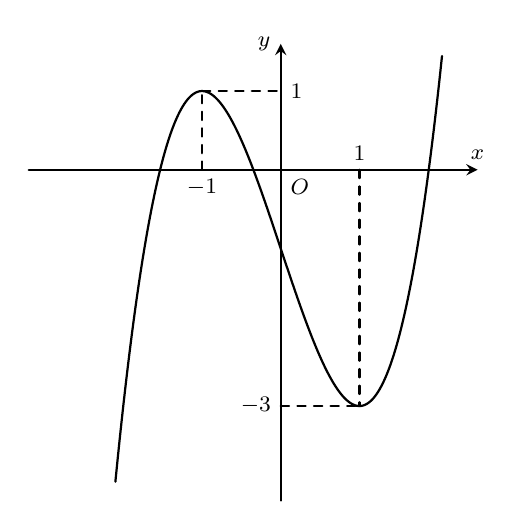
\begin{tikzpicture}[scale=1,font=\footnotesize, line cap=round,line join=round,>=stealth]
\draw[->, thick] (-3.2,0) -- (2.5,0) node[above] {$x$};
\draw[->, thick] (0,-4.2) -- (0,1.6) node[left] {$y$};
\draw[thick, smooth, domain=-2.1:2.05, samples=200]plot (\x, {\x*\x*\x - 3*\x - 1});
\draw[dashed, thick] (-1,0) -- (-1,1);
\draw[dashed, thick] (-1,1) -- (0,1);
\draw[dashed, thick] (1,0) -- (1,-3);
\draw[dashed, thick] (0,-3) -- (1,-3);
\node[below] at (-1,0) {$-1$};
\node[below right] at (0,0) {$O$};
\node[above] at (1,0) {$1$};
\node[right] at (0,1) {$1$};
\node[left] at (0,-3) {$-3$};
	\end{tikzpicture}
	 \end{center}
	
\choiceTF
{\True Hàm số đã cho nghịch biến trên khoảng $(-1;1)$}
{\True Hàm số đạt cực tiểu tại điểm $x_0=1$}
{\True Đạo hàm của hàm số nhận giá trị dương trên khoảng $(-\infty;-1)$}
{Giá trị nhỏ nhất của hàm số trên đoạn $[-1;0]$ bằng $-3$}
	\loigiai{
		\begin{itemchoice}
			\itemch \textbf{Đúng.} Trên khoảng $(-1;1)$ đồ thị có hướng đi xuống từ trái sang phải nê hàm số đã cho nghịch biến trên khoảng $(-1;1)$.
			\itemch \textbf{Đúng.} Hàm số đạt cực tiểu tại điểm $x_0=1$.
			\itemch \textbf{Đúng.} Trên $(-\infty;-1)$ đồ thị có hướng đi lên từ trái sang phải nên hàm số đồng biến. Do đó $f'(x)>0$.
			\itemch \textbf{Sai.} Giá trị nhỏ nhất của hàm số trên đoạn $[-1;0]$ khác $-3$.
		\end{itemchoice}
	}
\end{ex}
\Closesolutionfile{ans}

\Opensolutionfile{ans}[ans/ans-26-2-LangSon-SoGD-L1-KQ]
\caukq
\begin{ex}%[1H8V5-4]%Câu 1
	Cho hình lăng trụ đứng $ABC.A^\prime B^\prime C^\prime$ có đáy $ABC$ là tam giác vuông tại $A$, biết $AB=2$, $AC=3$, $AA^\prime=4$. Gọi $M$ là trung điểm của $AB$. Khoảng cách giữa hai đường thẳng $A^\prime B$ và $CM$ bằng bao nhiêu? \textit{(kết quả làm tròn đến hàng phần trăm)}.
	\shortans{$0{,}86$}
	\loigiai{
	\begin{center}
	\begin{tikzpicture}[scale=1,font=\footnotesize, line cap=round,line join=round,>=stealth]
\clip(-4.06,-3.02) rectangle (10.26,7.88);
\draw [thick](1.,1.)-- (1.,5.);
\draw [thick](1.,1.)-- (3.,0.);
\draw [thick,dashed](1.,1.)-- (6.,1.);
\draw [thick,->] (1.,5.) -- (1.,6.);
\draw [thick,->] (6.,1.) -- (7.,1.);
\draw [thick,->] (3.,0.) -- (5.,-1.);
\draw [thick](1.,5.)-- (6.,5.);
\draw [thick](1.,5.)-- (3.,4.);
\draw [thick](3.,4.)-- (6.,5.);
\draw [thick](3.,4.)-- (3.,0.);
\draw [thick](6.,5.)-- (6.,1.);
\draw [thick](3.,0.)-- (6.,1.);
\draw [thick, dashed](6.,1.)-- (1.976,0.512);
\draw [thick](1.,5.)-- (3.,0.);
\draw (0.44,1.3) node[anchor=north west] {$A$};
\draw (2.68,0.1) node[anchor=north west] {$B$};
\draw (5.7,1.1) node[anchor=north west] {$C$};
\draw (0.4,5.54) node[anchor=north west] {$A'$};
\draw (2.82,4.5) node[anchor=north west] {$B'$};
\draw (6.12,5.42) node[anchor=north west] {$C'$};
\draw (0.48,6.3) node[anchor=north west] {$z$};
\draw (4.78,-0.4) node[anchor=north west] {$x$};
\draw (6.7,1.76) node[anchor=north west] {$y$};
\draw (1.46,0.64) node[anchor=north west] {$M$};
\draw (0.26,3.18) node[anchor=north west] {$4$};
\draw (3.42,0.2) node[anchor=north west] {$2$};
\draw (6.06,1.76) node[anchor=north west] {$3$};
\end{tikzpicture}
	\end{center}
		Chọn hệ trục tọa độ $Oxyz$ sao cho $O$ trùng $A$, điểm $B\in Ox$, điểm $C\in Oy$. Khi đó $B(2;0;0)$, $C(0;3;0)$, $A'(0;0;4)$, $M(1;0;0)$.\\
		Ta có $\overrightarrow{A^\prime B} = (2;0;-4)$, $\overrightarrow{CM} = (1;-3;0)$, $\overrightarrow{MB}=(1;0;0)$. Suy ra $\left[\overrightarrow{A^\prime B},\overrightarrow{CM}\right]=(-12;-4;-6)$.\\
		Vậy $\mathrm{d}(A^\prime B,CN) = \dfrac{\left|\left[\overrightarrow{A^\prime B},\overrightarrow{CM}\right]\cdot\overrightarrow{MB}\right|}{\left|\left[\overrightarrow{A^\prime B},\overrightarrow{CM}\right]\right|}=\dfrac{(-12)\cdot 1-4\cdot 0-6\cdot 0}{\sqrt{(-12)^2+(-4)^2+(-6)^2}}=\dfrac{6}{7} \approx 0{,}86$.
	}
\end{ex}

\begin{ex}%[2H5V1-3]%Câu 2
	Trong không gian $Oxyz$, cho điểm $M(1;-2;-5)$. Gọi $(P)$ là mặt phẳng đi qua $M$ và cách gốc tọa độ một khoảng lớn nhất. Biết mặt phẳng $(P)$ cắt $Ox$, $Oy$, $Oz$ lần lượt tại ba điểm $A$, $B$, $C$. Thể tích tứ diện $OABC$ bằng bao nhiêu?
	\shortans{$450$}
	\loigiai{
	Gọi $H$ là hình chiếu vuông góc của $O$ lên mặt phẳng $(P)$. Khi đó $OH\leq OM$. Do đó, mặt phẳng $(P)$ cách gốc tọa độ lớn nhất khi $H\equiv M$ hay $\overrightarrow{OM}=(1;-2;-5)$ là vectơ pháp tuyến của $(P)$. Phương trình của mặt phẳng $(P)$ là $1(x-1)-2(y+2)-5(z+5)=0 \Leftrightarrow x-2y-5z-30=0$.\\
		Giao điểm của $(P)$ với các trục $Ox$, $Oy$, $Oz$ lần lượt là $A(30;0;0), B(0;-15;0), C(0;0;-6)$.\\
		Vậy thể tích khối tứ diện $OABC$ là $V = \dfrac{OA\cdot OB\cdot OC}{6}= \dfrac{30\cdot 15\cdot 6}{6}= 450$.
	}
\end{ex}

\begin{ex}%[2D4V1-6]%Câu 3
	Ở giai đoạn thải trừ, giai đoạn cuối sau khi một người uống một liều thuốc, nồng độ thuốc trong máu, ký hiệu là $C(t)$ (đơn vị: mg/l), giảm dần sau $t$ giờ kể từ khi giai đoạn này bắt đầu. Khi đó, tốc độ giảm nồng độ $C^\prime(t)$ tỉ lệ với chính nồng độ hiện có, tức là: $\dfrac{C^\prime(t)}{C(t)}=-k$ ($k$ là một hằng số dương). Biết rằng khi bắt đầu giai đoạn thải trừ, nồng độ thuốc còn lại là $12$ mg/l và sau $6$ giờ kể từ lúc bắt đầu thải trừ, nồng độ đo được là $3$ mg/l. Sau khoảng bao nhiêu giờ thì nồng độ còn lại bằng $2$ mg/l? (\textit{kết quả làm tròn đến hàng phần mười)}.
	\shortans{$7{,}8$}
	\loigiai{
Ta có $\dfrac{C^\prime(t)}{C(t)}=-k$. Suy ra $\displaystyle\int\dfrac{C^\prime(t)}{C(t)}dt=\int -kdt\Leftrightarrow \left|\ln C(t)\right|=-kt+D$ với $D\in\mathbb{R}$.\\
Cho $t=0$. Ta có $\left|\ln 12\right|=D\Leftrightarrow  D=\ln 12$.\\
Cho $t=6$. Ta có $\left|\ln 3\right|=-6k+\ln 12\Leftrightarrow k=\dfrac{\ln 2}{3}$.\\
Khi đó $C(t)=2\Rightarrow \left|\ln 2 \right|=-\dfrac{\ln 2}{3}\cdot t  \Leftrightarrow t=\dfrac{3\ln 6}{\ln 2}\approx 7{,}8$ 		
		}
\end{ex}

\begin{ex}%[0D8V1-3]%Câu 4
	Một màn chơi của một trò chơi điện tử được thiết kế như sau: có năm vị trí $A$, $B$, $C$, $D$, $E$, được đặt ở năm đỉnh của một hình chóp tứ giác. Nhân vật sẽ được đặt ở một vị trí bất kỳ, và có thể di chuyển tự do giữa các đỉnh với nhau, mỗi lần di chuyển đều phải từ đỉnh này di chuyển đến đỉnh khác. Giả sử khi bắt đầu, nhân vật được đặt ở vị trí $A$. Số cách di chuyển để sau sáu bước nhảy, nhân vật quay lại vị trí $A$ là bao nhiêu?
\begin{center}
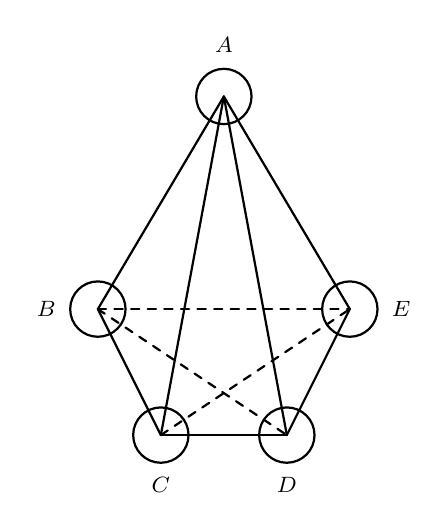
\begin{tikzpicture}[scale=1, font=\footnotesize, line join=round, line cap=round, >=stealth]
\coordinate (A) at (0,3.5);
\coordinate (B) at (-1.6,0.8);
\coordinate (C) at (-0.8,-0.8);
\coordinate (D) at (0.8,-0.8);
\coordinate (E) at (1.6,0.8);
%\draw[thick] (A) -- (B);
\draw [thick](A) -- (B);
\draw [thick](A) -- (C);
\draw [thick](A) -- (D);
\draw [thick](A) -- (E);
\draw [thick](B) -- (C);
\draw [thick](C) -- (D);
\draw [thick](D) -- (E);
\draw[thick, dashed] (B) -- (E);
\draw[thick, dashed] (B) -- (D);
\draw[thick, dashed] (C) -- (E);
\draw [thick](A)  circle (10pt);
\draw [thick](B)  circle (10pt);
\draw [thick](C)  circle (10pt);
\draw [thick](D)  circle (10pt);
\draw [thick](E)  circle (10pt);
\node[above=4pt] at (0,3.8) {$A$};
\node[left=6pt]  at (-1.8,0.8) {$B$};
\node[below=6pt] at (-0.8,-1) {$C$};
\node[below=6pt] at (0.8,-1) {$D$};
\node[right=6pt] at (1.8,0.8) {$E$};
\end{tikzpicture}
\end{center}	 
	 
	\shortans{$820$}
	\loigiai{
		Ký hiệu $a_n$ là số cách di chuyển để sau $n$ bước nhảy thì quay lại đỉnh $A$. Ký hiệu $x_n$ là số cách di chuyển để sau $n$ bước nhảy thì không quay lại đỉnh $A$.\\
		\textbf{Trường hợp $n=1$.} Ta có $a_1=0$, $x_1=4$.\\
		\textbf{Trường hợp $n=2$.} Ta có $a_2=x_1\cdot 1=4$, $x_2=x_1\cdot 3=12$.\\
		\textbf{Trường hợp $n=3$.} Ta có $a_3=x_2\cdot 1=12$, $x_3=3x_2+4a_2=52$.\\
		\textbf{Trường hợp $n=4$.} Ta có $a_4=x_3$, $x_4=3x_3+4a_3$.\\
		Như vậy ta có $\begin{cases}a_{n+1}=x_n\\x_{n+1}=2x_n+4a_n.\end{cases}$ Do đó $a_4=x_3=52$ và $x_4=3x_3+4a_3=204$.\\
		\textbf{Trường hợp $n=5$.} Ta có $a_5=x_4=204$ và $x_5=3x_4+4a_4=820$.\\
		\textbf{Trường hợp $n=6$.} Ta có $a_6=x_5=820$.

Vậy có $820$ cách di chuyển để sau $6$ bước, nhân vật quay lại đỉnh $A$.
	}
\end{ex}

\begin{ex}%[2D1V3-6]%Câu 5
	Một nhà máy sản xuất $x$ sản phẩm trong mỗi tháng. Chi phí sản xuất $x$ sản phẩm được cho bởi hàm chi phí $C(x)=16\,000+500x-1{,}6x^2+0{,}004x^3$ (nghìn đồng). Biết giá bán của mỗi sản phẩm là một hàm số phụ thuộc vào số lượng sản phẩm $x$ và được cho bởi công thức $p(x)=1\,700-7x$ (nghìn đồng). Hỏi mỗi tháng nhà máy nên sản xuất bao nhiêu sản phẩm để lợi nhuận thu được là lớn nhất? Biết rằng kết quả khảo sát thị trường cho thấy sản phẩm sản xuất ra sẽ được tiêu thụ hết.
	\shortans{$100$}
	\loigiai{
		Doanh thu $R(x) = x \cdot p(x) = 1\,700x - 7x^2$.\\
		Lợi nhuận $P(x) = R(x) - C(x) = -0{,}004x^3 - 5{,}4x^2 + 1\,200x - 1\,6000$.\\
		Ta có $P'(x) = -0{,}012x^2 - 10{,}8x + 1\,200$.\\
		$P'(x)=0 \Rightarrow -0{,}012x^2 - 10{,}8x + 1\,200 = 0 \Rightarrow x = 100$ hoặc $x = -1\,000$ (loại).\\

\begin{center}

\begin{tikzpicture}
\tkzTabInit[nocadre=false,lgt=1.2,espcl=2.5,deltacl=0.6]{$x$/1,$P'(x)$/1,$P(x)$/2}{$0$,$100$,$+\infty$}
\tkzTabLine{,+,0,-,}
\tkzTabVar{-/$-16\,000$,+/ $46\,000$/,-/$-\infty$}
\end{tikzpicture}
\end{center}

		Vậy nhà máy cần sản xuất $100$ sản phẩm thì có lợi nhuận lớn nhất.
	}
\end{ex}

\begin{ex}%[0D6V3-2]%Câu 6
	Tại chương trình \lq\lq Gian hàng khởi nghiệp\rq\rq của nhà trường, ban tổ chức mở một gian hàng \lq\lq Vòng quay may mắn\rq\rq, toàn bộ số tiền thu được sẽ được quyên góp vào quỹ \lq\lq Mùa xuân cho em\rq\rq. Luật chơi của gian hàng như sau: Một vòng quay được chia thành $40$ ô, có kích thước bằng nhau, gồm:
\begin{itemize}
\item[-] $1$ ô ghi \lq\lq Phần quà trị giá $200$ nghìn đồng\rq\rq.
\item[-] $4$ ô ghi \lq\lq Phần quà trị giá $50$ nghìn đồng\rq\rq.
\item[-] $10$ ô ghi \lq\lq Phần quà trị giá $20$ nghìn đồng\rq\rq.
\item[-] $25$ ô ghi \lq\lq Chúc bạn may mắn lần sau\rq\rq.
\end{itemize}
Mỗi lượt chơi, người chơi sẽ trả $25$ nghìn đồng để quay và nhận phần quà có trị giá tương ứng với ô mà mũi tên trên vòng quay chỉ vào. Hỏi trung bình, ban tổ chức thu được bao nhiêu nghìn đồng trên một lượt từ mỗi người chơi?
	\shortans{$10$}
	\loigiai{
	\begin{center}
		\begin{tabular}{|c|c|c|c|c|}
		\hline 
		Phần thưởng (nghìn đồng) & $200$ & $50$ & $20$ & $0$ \\ 
		\hline 
		Số lượng & $1$ & $4$ & $10$ & $25$ \\ 
		\hline 
		\end{tabular} 
	\end{center}
		$\overline{x} = \dfrac{200\cdot 1+50\cdot 4+20\cdot 10+0\cdot 25}{40} = \dfrac{600}{40} = 15$ nghìn đồng.\\
		Số tiền trung bình ban tổ chức thu được trung bình là $25 - 15 = 10$ nghìn đồng.
	}	
\end{ex}
\Closesolutionfile{ans}